\documentclass[11pt]{article}
\usepackage[margin=1in]{geometry}
\usepackage{fancyhdr}
\usepackage{graphicx}
\usepackage[utf8]{inputenc}
\usepackage[T1]{fontenc}
\usepackage{cite}
\usepackage{xcolor}
\usepackage{listings}
\usepackage{pdfpages}



\pagestyle{fancy}
\fancyhead{}
%\fancyfoot{}
	\fancyhead[L]{Commande de robot par BCI}
\fancyhead[R]{Rafael, Mathieu, Heloise}
%\fancyhead[C]{\thepage}

\renewcommand{\contentsname}{\huge{\textbf{Table des matières}}}

\lstdefinestyle{DOS}
{
    backgroundcolor=\color{black},
    basicstyle=\scriptsize\color{white}\ttfamily
}


\begin{document}

%Title

\begin{titlepage}
\begin{center}

\includegraphics[scale=0.5]{CentraleSupelec.jpeg}\\
\vfill
\line(1,0){400}\\[1mm]
\huge{\textsc{\textbf{Rapport TL SIR Commande de robot par interface cérébrale}}}\\[3mm]
\Large{\textbf{- Rafael ELLER CRUZ, Mathieu DAVIET, Heloise HUYGHUES DESPOINTES-}}\\[1mm]
\Large{promo 2018}\\[1mm]
\line(1,0){400}\\[1mm]

\vfill

\end{center}
\end{titlepage}

%%%Table of contents%%%

\tableofcontents
\thispagestyle{empty}
\cleardoublepage

\pagenumbering{arabic}

%%%Introduction%%%
\setcounter{page}{1}
\section{Introduction}

Lors de ses 11 séances de TL d'approfondissement, nous avons eu l'occasion de réaliser la commande du robot Khepera à partir de signaux provenant d'une interface cerveau machine (BCI). Ce projet nous a permis de mettre en pratique les connaissances que nous avons acquises lors des cours de la majeure Systèmes Interactifs et Robotiques et plus particulièrement celles des cours Modélisation et Analyse Spectrale, Robotique autonome et Programmation C++.\\

\noindent Deux robots Khepera, un système d'acquisition cérébrale et des signaux pré-enregistrés ont été mis à notre disposition pour ce projet.Le robot ne sera commandé que par 4 ordres: rester immobile, tourner à droite, tourner à gauche et avancer.\\

\noindent Notre travail à travers les séances et dans ce rapport est décomposé en 2 grandes étapes: l'extraction des commandes sur les signaux BCI et le contrôle du robot. Ces deux étapes sont ensuite réunies sous C++ grâce au framework ROS.


\cleardoublepage

%%%Extraction de la commande%%%

\section{Extraction de la commande du robot à partir des signaux cérébraux}

\subsection{Étude théorique}
egbfoaubgoabgoabogbaojbfaobfaob



\cleardoublepage

\subsection{Étude pratique}
\subsubsection{Démarche choisie pour l'extraction de commande}
\subsubsection{Création de données labellisées}
\subsubsection{Filtrage passe bande du signal}
\subsubsection{Lissage du signal}
\subsubsection{Choix de la commande}
\subsubsection{Synthèse et résultats}

\cleardoublepage

%%%Commande du robot%%%

\section{Commande du robot}

 	  
\subsection{Implémentation de l'interface avec le robot}
4 commandes possibles: avancer, tourner à droite, tourner à gauche et ne rien faire

A footnote \footnote{https://hal.archives-ouvertes.fr/}

You can see a duck in figure \ref{fig:duck}.

\begin{figure}[!h]
\centering
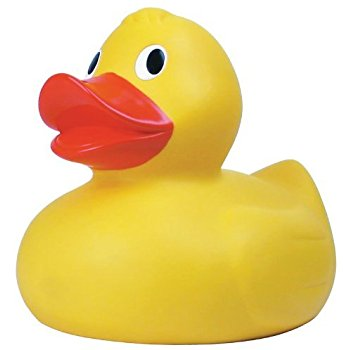
\includegraphics[scale=0.3]{bidon.jpg}
\caption{A duck}
\label{fig:duck}
\end{figure}

\cleardoublepage

\subsection{Adaptation de l'extraction du signal pour la commande du robots}

\cleardoublepage

\subsubsection{} \label{Deep}

	
\subsubsection{}

\cleardoublepage

%%%Analyse des résultats obtenus%%%

\section{Analyse des résultats}


\subsection{}

\subsection{Résultats et tests}

\cleardoublepage


%%%Synthèse des résultats%%%

\section{Synthèse des résultats}

\cleardoublepage

%%%Conclusion%%%

\section{Conclusion}
\cleardoublepage


%%%Annexe%%%

<<<<<<< HEAD
\section{Annexe}


\cleardoublepage

\end{document}
